\documentclass[a4paper]{article}
\usepackage{color}
\usepackage{indentfirst}
\usepackage{setspace}
\usepackage{tikz}
\usepackage{tikz-qtree}
\setlength{\parindent}{12pt}
\author{Chao Huang}
\title{COMP9319 Assignment 1}
\begin{document}
\maketitle


\section*{Question 1}
  \begin{spacing}{1.5}
    \noindent{}Given the text string below (note: it is banana not bananas below):\\
    \noindent{}bananainpajamas
    \begin{description}
      \item[a.] (5 Points) \textbf{What is its entropy?}\\
      \noindent{}When deal with the given string \textbf{bananainpajamas}, the character set S=\{a, b, i, j, m, n, p, s\} with frequency set \{6, 1, 1, 1, 1, 3, 1, 1\}. So the entropy of the string is:
      \[
        \sum_{i=1}^{n} -p(S_i)\log_2 {p(S_i)} = -\frac{6}{15}*\log_2 {\frac{6}{15}} - \frac{3}{15}*\log_2 {\frac{3}{15}} - 6 * \frac{1}{15}*\log_2 {\frac{1}{15}} = 1.25
      \]
      \item[b.] (5 Points) \textbf{Draw a Huffman tree based on the letters and their corresponding distributions for the above text string.}\\
      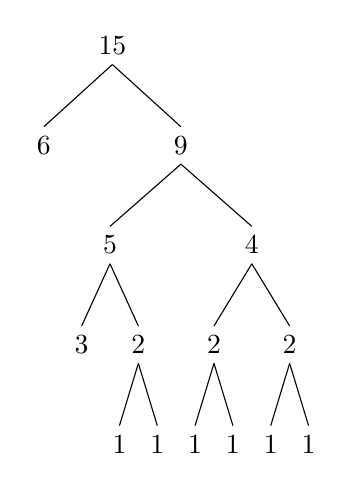
\begin{tikzpicture}[level distance=36pt]
        \Tree [.15 6 
                   [.9 [.5 
                         3 
                         [.2 1 1 ] 
                       ] 
                       [.4 
                         [.2 1 1 ]
                         [.2 1 1 ] 
                       ] 
                   ]
              ]
      \end{tikzpicture}
      \item[c.] (5 Points) \textbf{Provide the resulting Huffman code for each letter.}\\
      \noindent{}According to the Huffman tree, we get the code of each character:\\
      a: 0\\
      b: 1010\\
      i: 1011\\
      j: 1100\\
      m: 1101\\
      n: 100\\
      p: 1110\\
      s: 1111\\
      \item[d.] (5 Points) \textbf{What is the average number of bits needed for each letter, using your Huffman code? How does it compare to the entropy ? (i.e., equal/larger/small and why)}\\
      \noindent{} The average number of bits needed is 1.39, it is larger than the entropy, the cause of this situation is that: 
      \begin{description}
        \item[1.] Using Huffman coding to represent characters needs integral number of bits. This causes the increasing of number of bits we need to represent characters.
        \item[2.] When the frequency of some character is high, the non-optimality will emerge.
      \end{description}
    \end{description}
  \end{spacing}
  
\section* {Question 2}
  \begin{spacing}{1.5}
    \noindent{}\textbf{Adaptive Huffman Coding is used to encode a message source S, with a vocabulary of three letters a, b, c.}\\
    \textbf{The initial coding before any transmission is: a=00, b=01, c=10.}\\
    \textbf{Derive the encoded bitstream received from the decoder for the source message "abbcaab". Draw the adaptive Huffman trees after each of the additional letters is received.}\\\\
    \noindent{} The encoded bitstream is \textbf{000111011111}. And the Adaptive Huffman Tree will be as:
    \begin{center}
      
    \end{center}
  \end{spacing}
\section* {Question 3}
  \begin{spacing}{1.5}
    \begin{description}
      \item[a.] (10 Points) \textbf{The length of a source message is 8, containing letters a, b, c with their probability ranges as below:\\
      a [0.0, 0.2), b [0.2, 0.6), c [0.6, 1.0)\\
      Decode the arithmetic code 0.83 to its corresponding source message.}\\
      From the given probability ranges, we can get the table as:\\
      \begin{center}
        \begin{tabular}{ c c }
          New Character & Range \\
          \hline
          a & 0.00 - 0.20 \\
          b & 0.20 - 0.60 \\
          c & 0.60 - 1.00 \\
        \end{tabular}
      \end{center}
      The given arithmetic code 0.83 locates between 0.60 and 1.00, so we get the first character \textbf{c}.\\
      Then applying the arithmetic decoding to it.\\
      \begin{tabular} { c c c c c }
        Encoded Number & Output Symbol & Low & High & Range \\ \hline
        0.83 & c & 0.6 & 1.0 & 0.4 \\
        0.575 & b & 0.2 & 0.6 & 0.4 \\
        0.9375 & c & 0.6 & 1.0 & 0.4 \\
        0.84375 & c & 0.6 & 1.0 & 0.4 \\
        0.609375 & c & 0.6 & 1.0 & 0.4 \\
        0.0234375 & a & 0.0 & 0.2 & 0.2 \\
        0.1171875 & a & 0.0 & 0.2 & 0.2 \\
        0.5859375 & b & 0.2 & 0.6 & 0.4 \\
      \end{tabular}
      \item[b.] (10 Points) \textbf{Given that the source message is:\\
      banana\\
      Derive an arithmetic code. (Your answer should be in decimal number with minimum precision).}\\
      From the message \textbf{banana}, we can construct the table as below:\\
      \begin{center}
        \begin{tabular}{ c c c }
          New Character & Probability & Range \\ \hline
          a & $\frac{3}{6}$ & 0.0 - 0.5 \\
          b & $\frac{1}{6}$ & 0.5 - 0.67 \\
          n & $\frac{2}{6}$ & 0.67 - 1.0 \\
        \end{tabular}
      \end{center}
      Then we can derive another table from the one above as below:
      \begin{center}
        \begin{tabular}{ c c c }
          New Character & Low Value & High Value \\ \hline
            & 0.0 & 1.0 \\
          b & 0.5 & 0.667 \\
          a & 0.0 & 0.085 \\
          n & 0.72695 & 0.755 \\
          a & 0 & 0.014025 \\
          n & 0.67939675 & 0.684025 \\
          a & 0 & 0.002314125 \\
        \end{tabular}
      \end{center}
      From the table we can get the arithmetic code is 0.002314125.
    \end{description}
  \end{spacing}
\section*{Question 4}
  \begin{spacing}{1.5}
    \textbf{Consider the dictionary-based LZW compression algorithm. Suppose the alphabet is the set of ASCII characters, and the first 256 (i.e., $<$0$>$ to $<$255$>$) table entries are initialised to these characters.\\
    Show the dictionary (symbol sets plus associated codes) and output for LZW compression of the input (including the two spaces):\\
    nana likes banana\\}

  \end{spacing}
\section*{Question 5}
  \begin{spacing}{1.5}
    \begin{description}
      \item[a.] (8 Points) \textbf{Derive the Burrows Wheeler transform BWT(S) of character sequence S:\\
      bananainpajamas}\\
      \item[b.] (4 Points) \textbf{Derive the Move-to-Front transform of the BWT(S) from part (a), assuming we use the 255 ASCII symbols as the symbol table.}\\
      \item[c.] (8 Points) \textbf{Derive and recover the original character sequence S for the BWT(S):\\
      accc\$bbbaaaaaa\\
      where \$ is the pseudo end of sequence symbol (assume the sorting of these symbols is based on their ASCII representation).}\\
    \end{description}
  \end{spacing}
\end{document}
